\documentclass[a4paper,titlepage]{article}
\usepackage[utf8]{inputenc}
\usepackage[T1]{fontenc}
\usepackage[magyar]{babel}
\usepackage{amsmath}
\usepackage{float}
\usepackage{graphicx}

\newcommand{\Ai}[1]{\mathrm{Ai\left(#1\right)}}
\newcommand{\Bi}[1]{\mathrm{Bi\left(#1\right)}}
\newcommand{\Ti}[1]{\mathrm{Ti\left(#1\right)}}


\begin{document}
\section{Leírás}
	Kvantummechanikai iskolapélda a homogén térbe helyezett egydimenziós
	részecske. Ezt három dimenzióra kiterjesztve és két fal közé zárva
	keressük az energia sajátállapotokat. Annyi előrelátható, hogy a nyílt
	vagy félig nyílt esetekben használható, reguláris Airy függvény itt nem
	elegendő a megoldáshoz, ennyiben túlmegyünk a tankönyvi feladaton. Az
	aszimptotikus függvényalakok segítségével előállítjuk a magasan
	gerjesztett állapotok energiáit és hullámfüggvényeit, s ezeket
	összehasonlítjuk a közvetlenül a Bohr--Sommerfeld-módszerrel kapott
	eredménnyel. Numerikusan szemléltetjük fizikailag érdekes kezdőállapotok
	időfejlődését. Vizsgáljuk a rezolvenst és az állapotsűrűséget, továbbá a
	sokrészecske rendszerekre való általánosítás lehetőségét.
	
	Egydimenziós, $m$ tömegű, lineáris $F x$  potenciálban mozgó kvantumos részecskét zárjunk $L$ hosszú, merev falú dobozba (ekvivalens a padló és mennyezet között függőlegesen pattogó kvantum labdával).
	A stacionárius Schrödinger-egyenletből kiindulva, a határfeltételek figyelembe vételével, írjuk fel az energia sajátértékeket meghatározó szekuláris egyenletet, melyet oldjunk meg numerikusan. Ábrázoljuk az alacsonyabb nívókat a doboz méretének változtatása mellett, és szemléltessük grafikusan a stacionárius hullámfüggvényeket.  A szekuláris egyenletben fellépő függvények aszimptotikáinak ismeretében a magasabb nívókra próbáljunk egyszerűbb implicit formulát adni. Végezzük el a szemiklasszikus kvantálást is, hasonlítsuk össze az előző közelítő eredménnyel, és numerikusan néhány, az egzakt egyenletből kapott nívóval.

	További kérdések:  (a) Számítsuk ki a nívókat expliciten, kicsiny $L$-ek mellett. (b) Mely paraméterek mellett esik egybe $F L$ éppen az alapállapoti energiával?  (Ilyenkor a klasszikus labda éppen eléri a mennyezetet.)
	(c) Mutassuk meg, hogy e határesetnél kisebb $L$ belméret mellett minden nívó
	$F L$ fölé esik.
	(d) Írjuk fel a szemiklasszikus stacionárius hullámfüggvényeket, s grafikusan hasonlítsuk össze őket az egzaktakkal -- mikor jó a közelítés?
	(e) Írjuk fel a kicsiny L melletti hullámfüggvényeket expliciten, ezeket szintén hasonlítsuk össze a valódiakkal.
	
	-Miért nem Rodnik osztályba tartozik
	
	-20-as képlet lépcsőfüggvény
	
	-klasszikus út
	
	-fx, fy = 0 külön tárgyalás
	
	-program leírása
\section{Schrödinger}
	A probléma egy 1D dobozba zárt résecske homogén erőtérben. $F(x)=-F$, azaz $V(x) = Fx$.
	Az egyenlethez tartozó határfeltételek, ha a doboz hossza $L$:
	\begin{equation}
		\phi \big\rvert_0 = \phi \big \rvert_L = 0
	\end{equation}
	A megoldandó időfüggetlen Schrödinger-egyenlet:
	\begin{equation}
		-\frac{\hbar^2}{2m}\frac{d^2\phi}{dx^2} + Fx\phi = E\phi
	\end{equation}
	\begin{equation}
		\frac{d^2\phi}{dx^2} - \frac{2mFx}{\hbar^2}\phi = -\frac{2mE}{\hbar^2}\phi
	\end{equation}
	\begin{equation}
		\frac{d^2\phi}{dx^2} - \left(\frac{2mF}{\hbar^2}x - \frac{2mE}{\hbar^2}\right)\phi = 0
	\end{equation}
	Az Airy egyenlet ilyen alakra hozható a változó affin lineáris transzformációjával:
	\begin{equation}
		\frac{d^2y}{dx^{\prime 2}} - x^\prime y = 0
	\end{equation}
	$x^\prime = ax - bE$, azaz $\frac{d}{dx} = a\frac{d}{dx^\prime}$:
	\begin{equation}
		\frac{d^2y}{dx^2} - \left(a^3x - a^2bE\right)y = 0
	\end{equation}
	Az együtthatók összevetése alapján $a = \sqrt[3]{\frac{2mF}{\hbar^2}}$ és $b = \sqrt[3]{\frac{2m}{\hbar^2F^2}}$. Így a Schrödinger-egyenlet megoldása:
	\begin{equation}
		\phi(x) = y(x^\prime) = y\left(\sqrt[3]{\frac{2mF}{\hbar^2}}x - \sqrt[3]{\frac{2m}{\hbar^2F^2}}E\right)
	\end{equation}
	, ahol $y(x) = \alpha \Ai\left(x\right) + \beta \Bi\left(x\right)$.
	A $\phi \big\rvert_0 = 0$ feltételből következik, hogy $\phi \propto \Bi\left(-bE\right)\Ai\left(ax-bE\right) - \Ai\left(-bE\right)\Bi\left(ax-bE\right)$. A második határfeltétel pedig meghatározza a lehetséges energiákat. A feltétel:
	\begin{equation}
		\Bi\left(-bE\right)\Ai\left(aL-bE\right) - \Ai\left(-bE\right)\Bi\left(aL-bE\right) = 0
	\end{equation}
	\begin{equation}
		\label{box_energiaszintek_egyenlet}
		\Ti{aL-bE} - \Ti{-bE} = 0
	\end{equation}
	\begin{equation}
		\Ti{\sqrt[3]{\frac{2mF}{\hbar^2}}L - \sqrt[3]{\frac{2m}{\hbar^2F^2}}E} - \Ti{-\sqrt[3]{\frac{2m}{\hbar^2F^2}}E} = 0
	\end{equation}
	\begin{figure}[H]
		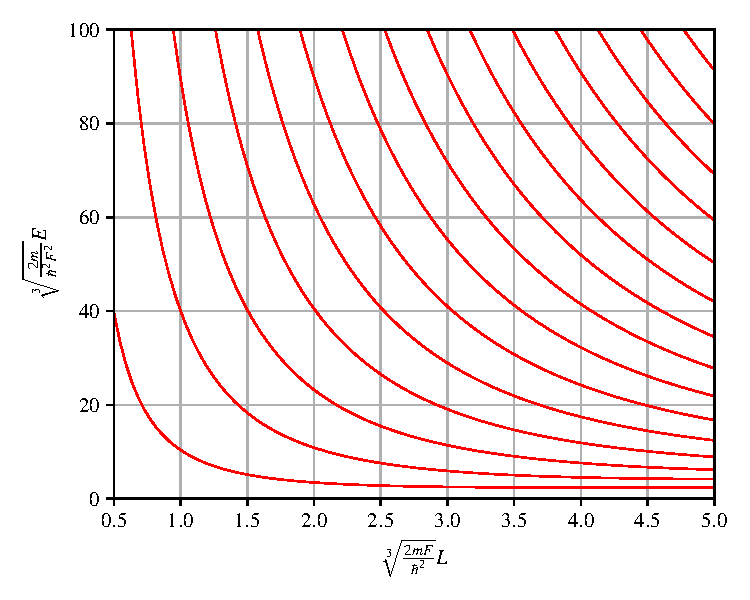
\includegraphics[scale=1]{./figs/energiaszintek.pdf}
		\caption[Egzakt energiaszintek]{Egzakt energia szintek, $bE$ és $aL$ közötti relációval ábrázolva. Az ába jobb alsó sarkán látható, hogy $E \ll FL$ esetén az energiaszintek $L$-től függetlenek lesznek, mivel a félvégtelen tér beli homogén tér energiaszintjeit közelítik.}
		\label{box_energiaszintek_abra}
	\end{figure}
	Amikor $FL \ll \frac{\pi^2\hbar^2}{2mL^2}$, a potenciál jól közelíthető konstans potenciállal, mivel az alapállapot energiájához képest is elhanyagolható a lineáris potenciál eltérése a konstans potenciáltól. Eben a esetben $E \propto n^2$. $E \ll FL$ esetben az energiaszintek jó közelítéssel konstanssá válnak. Ennek az oka, hogy $\lim_{L \to \infty}\psi(x) = \alpha \Ai\left(ax-b\right)$, mert a $\Bi\left(x\right)$ exponenciálisan növekszik nagy $x$-ek esetén. Ebben az eseten az energiaszinteket a $\Ai\left(- \sqrt[3]{\frac{2m}{\hbar^2F^2}}E\right) = 0$ egyenlet határozza meg. Ezeket az aszimptotikus viselkedéseket \aref{box_energiaszintek_abra}. ábra jól mutatja.
    
    TODO: link 1D videóról


\section{Kvantumos közelítése}
	\Aeqref{box_energiaszintek_egyenlet} egyenletet nagy $bE$ illetve nagy $bE-aL$ esetén \aeqref{airy:tiapprox} közelítés alkalmazható,
\begin{equation}
	\ctg\left(\frac{2}{3}\left(bE-aL\right)^{3/2}-\frac{\pi}{4}\right)-\ctg\left(\frac{2}{3}\left(bE\right)^{3/2}-\frac{\pi}{4}\right)=0.
	\label{quantumApprox:cot}
\end{equation}
A $\ctg(x)$ függvény $\pi$-ben periodikus, és mivel a $(0,\pi)$ intervallumban szigorúan monoton csökken, \aeqref{quantumApprox:cot} egyenletnek csak akkor van megoldása, ha a $\ctg(x)$ függvények argumentumainak különbsége $n\pi$, azaz
\begin{equation}
	\frac{2}{3}\left(bE\right)^{3/2}-\frac{2}{3}\left(bE-aL\right)^{3/2}=n\pi.
\end{equation}
Az $a$ és $b$ állandók behelyettesítésével ez az egyenlet \aeqref{semiclassicallevels:e2} egyenletet adja. Az $n$  értéke ugyan különbözik $1$-gyel a két egyenletben a Maslov indexek miatt, viszont mivel $n$ egész, ugyan azokat az energiaszinteket határozzák meg. Ennek nem feltétlenül kéne így lennie, viszont ebben az esetben a szemiklasszikus illetve az Airy-függvények aszimptotikus alakjából kapott közelítések egzaktul megegyeznek.

Amennyiben $bE-aL$ negatív, a $\Ti(bE-aL)$ gyorsan lecseng, \aeqref{quantumApprox:cot} egyenlet bal oldalának első tagja elhanyagolható. Ennek a tagnak az elhanyagolásával \aeqref{semiclassicallevels:e1} egyenletet kapjuk vissza. Ez a képlet felel meg az $L\to\infty$ határesetnek, ami a féltérben pattogó labdát írja le.

%$x \to \infty$ aszimptotikus alak:
%	\begin{equation}
%		\Ai\left(-x\right) = \frac{1}{\sqrt{\pi}x^{1/4}}\cos\left(\frac{2}{3}x^{3/2} - \frac{\pi}{4}\right) + \mathcal{O}\left(x^{-5/4}\right)
%	\end{equation}
%	\begin{equation}
%		\Bi\left(-x\right) = -\frac{1}{\sqrt{\pi}x^{1/4}}\sin\left(\frac{2}{3}x^{3/2} - \frac{\pi}{4}\right) + \mathcal{O}\left(x^{-5/4}\right)
%	\end{equation}
%	\begin{equation}
%		\Ti\left(-x\right) = -\cot\left( \frac{2}{3}x^{3/2} - \frac{\pi}{4} \right) + \mathcal{O}\left(x^{-5/4}\right)
%	\end{equation}
%	
%	Ezzel a közelítéssel \aref{box_energiaszintek_egyenlet}. egyenlet alakja:
%	\begin{equation}
%		\cot\left(\frac{2}{3}\left(bE-aL\right)^{3/2} - \frac{\pi}{4}\right) = \cot\left(\frac{2}{3}\left(bE\right)^{3/2} - \frac{\pi}{4}\right)
%	\end{equation}
%	, azaz
%	\begin{equation}
%		\frac{2}{3}\left(bE\right)^{3/2} - \frac{2}{3}\left(bE-aL\right)^{3/2} = n\pi
%	\end{equation}
%	. Az $a$ és $b$ behelyettesítésével az egyenlet
%	\begin{equation}
%		\frac{2\sqrt{2m}}{3F\hbar}\left(E^{3/2} - \left(E - FL\right)^{3/2}\right) = n\pi
%	\end{equation}
%	Ez megegyezik a szemiklasszikus kvantálással kapott eredménnyel, ami azt jelenti, hogy a szemiklasszikus közelítés jól működik nagy energiáknál, hibája $\mathcal{O}\left(E^{-5/4}\right)$ nagyságrendű.


\section{Szemiklasszikus}
	\begin{equation}
		nh = \oint p \, dq = 
	\end{equation}
	$E/F < L$ esete:
	\begin{equation}
		2\int_0^{E/F}\sqrt{2m\left( E-Fx \right)}\,dx = -\frac{2}{3mF}\left(2m\left( E-Fx \right)\right)^{\frac{3}{2}}\bigg \rvert_0^{E/F} = \frac{4\sqrt{2m}E^{3/2}}{3F}
	\end{equation}
	\begin{equation}
		E_n = \left(\frac{3nhF}{4\sqrt{2m}}\right)^{2/3}
	\end{equation}
	$E/F > L$ esete:
	\begin{equation}
		-\frac{2}{3mF}\left(2m\left( E-Fx \right)\right)^{\frac{3}{2}}\bigg \rvert_0^{L} = \frac{4\sqrt{2m}}{3F}\left(E^{3/2} - \left(E - FL\right)^{3/2}\right) = nh
	\end{equation}
	$E \gg FL$ esetén a különbség az $E^{3/2}$ függvény deriváltjának segítségével helyettesíthető:
	\begin{equation}
		nh \approx 2\sqrt{2m}E^{1/2}L
	\end{equation}
	\begin{equation}
		E_n \approx \frac{n^2h^2}{8mL^2}
	\end{equation}
	
	\begin{figure}[H]
		\centering
		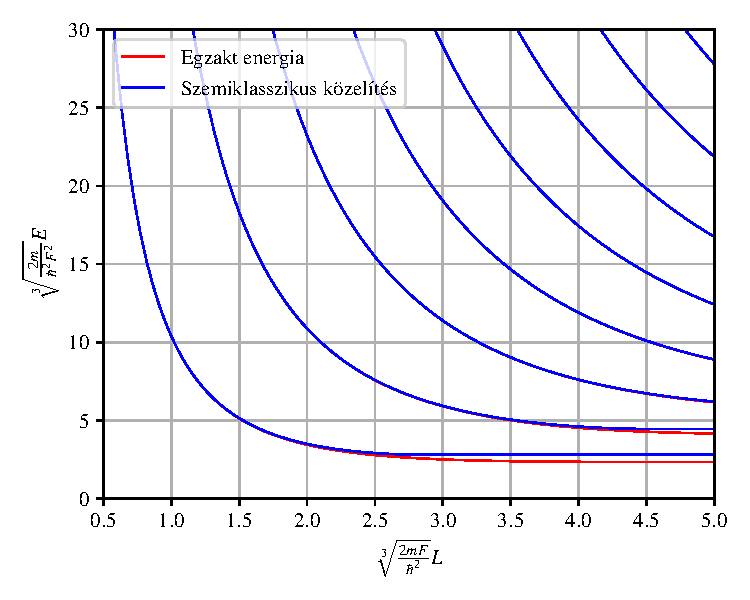
\includegraphics[scale=1]{./figs/energiaszintkozelites.pdf}
		\caption[Szemiklasszikus energiaszintek]{Az ábra a szemiklasszikus energiaszinteket hasonlítja össze az egzakt energiaszintekkel. Ez az ábra is a $bE$ és $aL$ közötti relációt ábrázolja. A szemiklasszikus közelítés nagy kvantumszámok illetve $E \gg FL$ esetén pontos. Utóbbi oka, hogy ebben az esetben a potenciál elhanyagolható, és a potenciál nélküli végtelen potenciálgödör energiaszintjeit pedig a szemiklasszikus közelítés egzaktul megadja.}
	\end{figure}
	
	\begin{figure}[H]
		\centering
		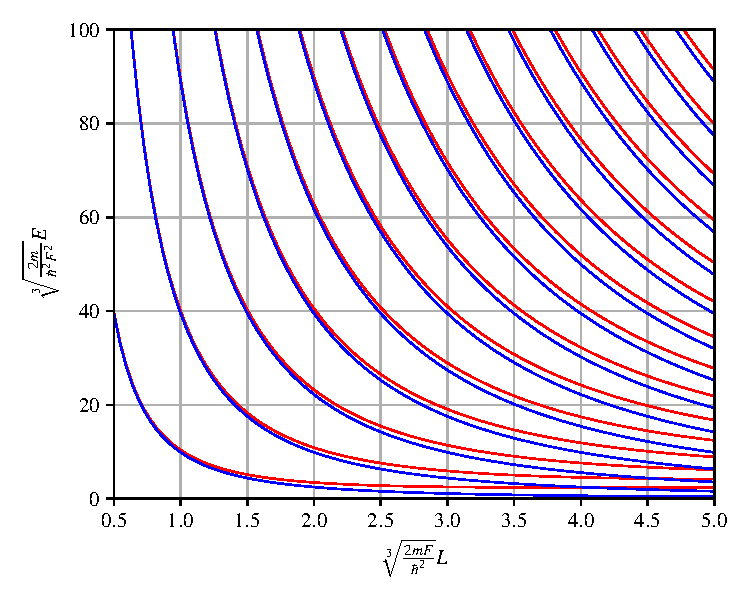
\includegraphics[scale=1]{./figs/infsquareenergia.pdf}
		\caption[Végtelen potenciálgödör energiaszintjei]{Az ábrán a végtelen potenciálgödör és az egzakt energiaszintek összehasonlítása látható. Ez csak az $E \gg FL$ esetben jó közelítés, a szemiklasszikus energiaszintek jóval pontosabbak.}
	\end{figure}


\section{Momentumok}
	\input{momentum.tex}
	
\section{Plafon érintés 1D}
	Azokat a parmaétereket keresem, ahol az alapállapot $E = FL$:
	\begin{equation}
		\Ti{\sqrt[3]{\frac{2mF}{\hbar^2}}L - \sqrt[3]{\frac{2m}{\hbar^2F^2}}FL} - \Ti{-\sqrt[3]{\frac{2m}{\hbar^2F^2}}FL} = 0
	\end{equation}
	, azaz
	\begin{equation}
		\Ai{-\sqrt[3]{\frac{2mF}{\hbar^2}}L} = 0
	\end{equation}
	. Az első gyöke az Airy függvénynek megadja azt az esetet, amikor az alapállapot ergiája $FL$, és nem pedig valamelyik gerjesztett állapoté.
	\begin{equation}
		-a_1 = \sqrt[3]{\frac{2mF}{\hbar^2}}L \approx 2.338
	\end{equation}



\section{3D doboz, ferde tér}
    A rendszer egy téglatest alakú dobozba zárt részecske. A doboz mérete $L_x$, $L_y$ és $L_z$. A dobozban homogén erőtér hat a részecskére, azaz $\boldsymbol{F} = \text{const}$. A potenciál így $V(x, y, z) = -F_xx-F_yy-F_zz$. A rendszer időfüggő Schrödinger-egyenlete
\begin{equation}
	i\hbar\frac{\partial \psi(x, y, z, t)}{\partial t} = -\frac{\hbar^2}{2m} \Laplace \psi(x, y, z, t) + V(x, y, z)\psi(x, y, z, t).
	\label{3dbox:3dscheq}
\end{equation}
Az egyenlet kezdőfeltétele egy kezdeti állapot $t_0$-ban, $\psi(x, y, z, t_0) = \psi_0(x, y, z)$, az egyenlet határfeltételei pedig a hullámfüggvény határokon való eltűnése, $0=\left.\psi\right|_{x=0}=\left.\psi\right|_{x=L_x}=\left.\psi\right|_{y=0}=\left.\psi\right|_{y=L_y}=\left.\psi\right|_{z=0}=\left.\psi\right|_{z=L_z}$. Mivel ez a potenciál lineáris $x$, $y$ és $z$-ben, a Schrödinger-egyenlet szeparálható a
\begin{equation}
	\psi_{klm}(x, y, z, t) = e^{-\frac{iE_{klm}}{\hbar}t}\psi^{(1)}_k(x)\psi^{(2)}_l(y)\psi^{(3)}_m(z)
	\label{3dox:3dansatz}
\end{equation}
próbafüggvénnyel. A $\psi^{(i)}_n$ függvényekre így az egy dimenziós stacionárius Schrödinger-egyenlet vonatkozik. A $\psi^{(i)}$-re vonatkozó egyenlet 
\begin{equation}
	-\frac{\hbar^2}{2m}\frac{d^2\psi^{(i)}_k(x_i)}{dx_i^2} + F_ix_i\psi^{(i)}_k(x) = E^{(i)}_k\psi^{(i)}_k(x_i),
	\label{3dbox:1deq}
\end{equation}
a határfeltételek $\left.\psi^{(i)}_k\right|_{x_i=0}=\left.\psi^{(i)}_k\right|_{x_i=L_i}=0$. Az $E_{klm}$ energia a három egy dimenziós stacionárius Schrödinger-egyenlet sajátenergiáinak összege,
\begin{equation}
	E_{klm} = E^{(1)}_k+E^{(2)}_l+E^{(3)}_m.
\end{equation}
\Aeqref{3dbox:3dscheq} egyenlet általános megoldása \aeqref{3dox:3dansatz} próbafüggvények kezdőfeltételhez illesztett lineáris kombinációja,
\begin{equation}
	\psi(x,y,z,t) = \sum_{klm}C_{klm}\psi_{klm}(x,y,z,t).
	\label{3dbox:timeevolution}
\end{equation}
$C_{klm}$ együtthatók meghatározásához a szokásos hely reprezentáció beli skalárszorzást kell használni,
\begin{equation}
	C_{klm} = \frac{1}{N_{klm}}\int_0^{L_x}dx\int_0^{L_y}dy\int_0^{L_z}dz\,\psi_{klm}(x, y, z, t=0)^*\psi_0(x, y, z),
	\label{3dbox:ceq}
\end{equation}
\begin{equation}
	N_{klm} = \int_0^{L_x}dx\int_0^{L_y}dy\int_0^{L_z}dz\,|\psi_{klm}(x,y,z,t=0)|^2.
	\label{3dbox:3norm}
\end{equation}
\Aeqref{3dbox:ceq} egyenlet nem egyszerűsíthető tovább általános $\psi_0$ esetén, viszont \aeqref{3dbox:3norm} igen. Mivel $\psi_{klm}$ szorzat alakú, nem kell a tripla integrált elvégezni, elég csak három egyszeres integrál szorzatát kiszámítani. Ez numerikus számításokban jelentős.
\begin{equation}
	N_{klm} = N^{(x)}_kN^{(y)}_lN^{(z)}_m,
\end{equation}
ahol az egyes $N$ tagok az egy dimenziós sajátfüggvények normájaként vannak definiálva.
\begin{equation}
	N^{(i)}_k = \int_0^{L_i}dx_i\,\left|\psi^{(i)}_k(x_i)\right|^2.
\end{equation}
A továbbiakban az egy dimenziós probléma részleteit vizsgáljuk.

%    TODO: ÁBRA AZ EGYSZER FÜGGŐLEGES ESET ENERGIÁIRÓL, esetleg szintén L függvényében.
%    
%    TODO: ábra 2D -quantum chaos in billiards-
%    
%    TODO: 2D (3D?) videó link időfelődésről

    
\section{Green függvény}
    
\section{Videó gyártás leírása}
    
    
    
\end{document}















